% ===========================================================================
\section{Extension: spatial curvature}\label{sec:curvature}
% ===========================================================================

The milestones assume a flat universe. As an extension we added spatial curvature to all modules. Curvature is
one of the main targets of the CMB: it changes the distance to the last-scattering surface, and therefore the angle
under which the acoustic scale appears. Throughout this section the matter, radiation and baryon densities are those
of the fiducial model, and $\Om_{\Lambda0}=1-\Om_{M0}-\Om_{r0}-\Om_{K0}$ absorbs the change.

\subsection{Theory}

\paragraph*{Background.} With $K=-\Om_{K0}H_0^2/c^2$ ($K<0$ open, $K>0$ closed), the Friedmann equation already
contains the curvature term $\Om_{K0}e^{-2x}$. Distances use the comoving transverse distance
$r=\sin_K(\chi)\equiv\sin(\sqrt K\chi)/\sqrt K$, $\chi$, or $\sinh(\sqrt{-K}\chi)/\sqrt{-K}$ for closed, flat and open
space. In a closed universe light rays from a point converge again, so objects at fixed $\chi$ look larger; in an open
universe they diverge and objects look smaller.

\paragraph*{Perturbations.} In curved space the plane waves $e^{i\bm k\cdot\bm x}$ are replaced by eigenfunctions of
the Laplacian, $\nabla^2G=-k^2G$. It is convenient to label them by $q^2=k^2+K$ and $\nu=q/\sqrt{|K|}$. In an open
universe every $q>0$ is allowed. A closed universe is finite, so the spectrum is discrete: only integer $\nu\ge3$
describe scalar perturbations ($\nu=1$ is a homogeneous change of the background and $\nu=2$ is a pure gauge
mode). Three changes follow in the equations of
Milestone~III~\cite{HuSeljak1998,Lesgourgues2014}:
\begin{itemize}
\item The $00$ Einstein equation contains $k^2-3K$ instead of $k^2$: curvature adds to the potential energy of a
      perturbation. The same factor appears in the Poisson equation for $\Delta_M$.
\item The free-streaming couplings between neighbouring multipoles of photons, polarization and neutrinos carry the
      factors $s_\ell=\sqrt{1-(\ell^2-1)K/k^2}$:
      $\Theta_\ell'=\frac{\kappa}{2\ell+1}[\ell s_\ell\Theta_{\ell-1}-(\ell+1)s_{\ell+1}\Theta_{\ell+1}]+\dots$. Geometrically,
      the angle subtended by a wavelength changes along the line of sight. In a closed universe $s_\nu=0$, so the
      hierarchy of mode $\nu$ ends at $\ell=\nu-1$: a finite space has no structure on angles smaller than its modes
      allow. In this convention the physical shear is $\Theta_2/s_2$, which enters $\Psi$.
\item The truncation of the hierarchies uses $\cot_K(\eta)$ instead of $1/\eta$.
\end{itemize}
The initial conditions are those of the flat case, since curvature is negligible at $x=-18$, and we keep the
normalization $\mathcal{R}=1$ and $\mathcal{P}_{\mathcal{R}}=A_s(k/k_{\rm pivot})^{n_s-1}$, as in CLASS.

\paragraph*{Hyperspherical Bessel functions.} The projection of a mode onto the sky now uses the radial
eigenfunctions $\Phi^\nu_\ell(\chi)$ (with $\chi$ in units of the curvature radius) instead of $j_\ell(kr)$. They obey
\begin{equation}
\Phi''+2\cot_K\chi\,\Phi'+\Big[\nu^2-{\rm sgn}K-\frac{\ell(\ell+1)}{\sin_K^2\chi}\Big]\Phi=0,
\end{equation}
with $\Phi^\nu_0=\sin(\nu\chi)/(\nu\sin_K\chi)$ and the three-term recurrence
\begin{align}
\sqrt{\nu^2-{\rm sgn}K(\ell+1)^2}\,\Phi_{\ell+1} &= (2\ell+1)\cot_K\chi\,\Phi_\ell \nonumber\\
 &\quad -\sqrt{\nu^2-{\rm sgn}K\,\ell^2}\,\Phi_{\ell-1}.
\end{align}
They reduce to $j_\ell(\nu\chi)$ for $\nu\to\infty$. The line-of-sight integral no longer allows the integrations by
parts used in Eq.~\eqref{eq:ST}, so we project the three parts of the source separately:
\begin{align}
\Theta_\ell(k) &= \int\dd x\,\Big[S_{T0}\Phi_\ell + S_{T1}\frac{\sqrt{|K|}}{k}\Phi_\ell' \nonumber\\
 &\qquad + S_{T2}\frac{3(|K|/k^2)\Phi_\ell''+\Phi_\ell}{2s_2}\Big],\\
\Theta^E_\ell(k) &= \sqrt{\tfrac{(\ell+2)!}{(\ell-2)!}}\int\dd x\,\frac{3\gt\,\Pi}{4}\,\frac{\Phi_\ell}{s_2(kr)^2},
\end{align}
with $S_{T0}=\gt(\Theta_0+\Psi)+e^{-\tau}(\Psi'-\Phi')$, $S_{T1}=-\gt v_b$ and $S_{T2}=\gt\Pi/2$. In the flat limit
these are $j_\ell$, $j_\ell'$ and $(3j_\ell''+j_\ell)/2$, and integrating by parts recovers Eq.~\eqref{eq:ST}. In a
closed universe the $k$-integral of Eq.~\eqref{eq:cl} becomes a sum over integer $\nu$.

\subsection{Implementation and tests}

$\Phi^\nu_\ell$ is computed by upward recurrence~\cite{Kosowsky1998,Tram2017} below the turning point
$\ell(\ell+1)=(\nu^2-{\rm sgn}K)\sin_K^2\chi$, where it oscillates, and by Miller's downward recurrence above it, where
it decays exponentially; in a closed universe the downward recurrence starts exactly at $\ell=\nu-1$. The functions
agree with $j_\ell$ in the flat case to $2\times10^{-12}$, satisfy the radial equation to the accuracy of the finite
differences, match the closed-form Gegenbauer polynomials of a closed universe to $10^{-13}$, and approach
$j_\ell(\nu\chi)$ as $1/\nu^2$.

The perturbations are sampled in $q$; in a closed universe only integer $\nu$ are used, and in an open universe the
grid extends down to $q=0.01\sqrt{|K|}$, since the modes near the curvature scale contribute to the lowest multipoles.
For each mode and each point on the line of sight we compute $\Phi_0\dots\Phi_{\ell_{\rm cap}}$, where $\ell_{\rm cap}$ is
just beyond the turning point. One subtlety concerned the closed-universe sum. Rounding a uniform $k$-grid to integer
$\nu$ gives an irregular stride of 2--3 in $\nu$, while $\Theta_\ell^2$ oscillates with a period of only a few units of
$\nu$. The trapezoidal rule then loses the high accuracy it has for oscillating integrands on a uniform grid, and $C_\ell$
was off by up to $4\%$. A uniform integer stride fixes this. With the flat Bessel functions the same code reproduces the
integrated-by-parts flat result to $5\times10^{-5}$, which tests the decomposition of the source. Two speed-ups bring the curved
line-of-sight integration from $\approx48$\,s to 26--42\,s on two cores for $\ell\le2000$ (7\,s with the flat
tables). First, modes with smaller $q$ use a proportionally coarser $x$-grid away from recombination (the radial
functions oscillate more slowly), but never coarser than $\Delta x=0.01$, which resolves reionization; this changes
$C_\ell$ by $<3\times10^{-5}$. Second, for $\nu\ge4000$ we use the flat approximation of CLASS: $\Phi^\nu_\ell(\chi)$ is
replaced by $j_\ell$ with the argument rescaled to put its turning point at $\chi_{\rm tp}$ and an empirical amplitude
correction~\cite{Lesgourgues2014}, read from tables of $j_\ell$ and $j_\ell'$. It is accurate near the turning point
but drifts in phase far beyond it. Since those oblique projections carry little weight for Silk-damped modes, the
effect on $C_\ell$ is $\lesssim6\times10^{-4}$ at $\Om_K=\pm0.05$, where a third of the modes use it. For
$|\Om_K|=0.2$ no mode reaches $\nu=4000$ below $k=0.3\Mpc^{-1}$, and lowering the threshold quickly costs accuracy
($0.4\%$ for $\nu\ge2000$, $1\%$ for $\nu\ge1000$).

\subsection{Results}

\begin{figure}
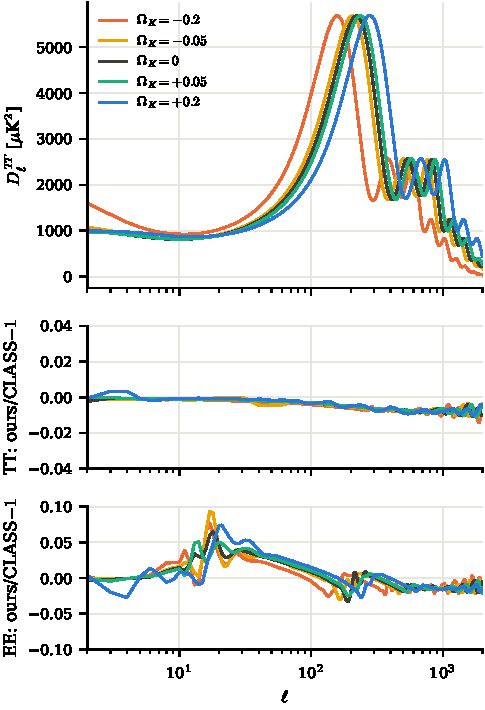
\includegraphics[width=\columnwidth]{curvature_spectra}
\caption{\emph{Top:} TT spectra for $\Om_K=-0.2$, $-0.05$, 0, 0.05 and 0.2 at fixed matter and baryon density.
\emph{Middle and bottom:} TT and EE relative to CLASS run with the same physics (unlensed).}
\label{fig:curvature}
\end{figure}

\begin{table}
\caption{Curved models: the first TT peak from our code and from CLASS, the acoustic scale $\ell_A=\pi r(\chi_*)/r_s$,
and the largest TT difference from CLASS for $30\le\ell\le2000$.}
\label{tab:curvature}
\begin{ruledtabular}
\begin{tabular}{rcccccc}
$\Om_K$ & $\Om_\Lambda$ & $\ell_{\rm peak}$ & CLASS & $\ell_A$ & $\ell_{\rm peak}/\ell_A$ & TT diff. \\
\hline
$-0.20$ & 0.883 & 158 & 158 & 215.7 & 0.732 & 1.4\% \\
$-0.05$ & 0.733 & 206 & 206 & 280.8 & 0.734 & 1.1\% \\
$0$     & 0.683 & 221 & 221 & 301.7 & 0.733 & 1.1\% \\
$+0.05$ & 0.633 & 236 & 236 & 322.2 & 0.733 & 1.2\% \\
$+0.20$ & 0.483 & 279 & 280 & 381.4 & 0.731 & 1.0\% \\
\end{tabular}
\end{ruledtabular}
\end{table}

Figure~\ref{fig:curvature} and Table~\ref{tab:curvature} show the result. Our spectra agree with CLASS as well in
curved as in flat models: TT to $0.15$--$0.35\%$ for $\ell\le30$ and $1$--$1.4\%$ up to $\ell=2000$, EE to $2$--$3\%$ for
$\ell\ge100$, and $P(k)$ to $0.12\%$ for $k>10^{-3}\Mpc^{-1}$ ($\Om_K=\pm0.05$). The background agrees to $10^{-6}$ and the potentials
today to $\sim10^{-5}$. The remaining differences are the same as in the flat case and come from the recombination
model.

The main effect of curvature is geometric. The physics at recombination is unchanged, because curvature is negligible
then, so the sound horizon is the same in all models to $0.05\%$ ($r_s=144.82$--$144.89\Mpc$; the small spread comes
from the optical depth to reionization, which shifts the $\tau=1$ surface). What changes is the transverse distance to the last-scattering surface, $r(\chi_*)$: it is
smaller in a closed universe, where light rays focus, and larger in an open one. The whole acoustic pattern therefore
shifts in $\ell$. The ratio $\ell_{\rm peak}/\ell_A$ is $0.731$--$0.734$ in all five models, so the first peak follows the
geometric prediction, while $\Om_K=\mp0.2$ moves it by $-29\%$ and $+26\%$. A measurement of the peak positions
therefore measures $r(\chi_*)/r_s$, which is why the CMB constrains curvature so well once $\Om_Mh^2$ is fixed by the
peak heights.

The low multipoles change too. In the closed model with $\Om_K=-0.2$ the larger $\Om_\Lambda=0.88$ makes the potentials
decay earlier and more strongly, and the late ISW effect raises $D_2$ to $1600\muK$ against $1020\muK$ in the flat
model. In the open models the opposite change in $\Om_\Lambda$ is partly compensated by curvature itself, which also
makes the potentials decay once it dominates the expansion. These large-scale effects are limited by cosmic variance,
and in practice the geometric degeneracy between $\Om_K$ and $\Om_\Lambda$ is broken by combining the CMB with
lensing or BAO.
